\addtocontents{toc}{\protect\newpage}
\chapter{Prototype}
In this chapter the development of the prototype is described.
This prototype will be delivered to the Zebro team, so should conform to all the interface requirements given in chapter~\ref{chap:por}.
The first step is to integrate the transmitter and receiver circuits and design the necessary power circuitry.
The next step is to link our distance measurement system to the communication system \cite{communication} and the processing system \cite{processing}.
Before we order the prototype PCB of the full system we test the systems on a naked prototype PCB produced with the PCB milling machine of the Zebro team.
This naked prototype PCB allows us to test if the systems will work on a PCB with surface-mounted devices (SMD) components.

Using the naked prototype PCBs we will test the prototype module in phases.
The test phases are described at the end of this chapter in section \ref{sec:testplan}.
The test results will be given in Chapter~\ref{chap:results}.

\section{Subsystem integration}

\subsection*{Switching between transmitting and receiving}

To integrate the receiver and transmitter circuit a switching circuit is required as shown in the overview in figure~\ref{fig:ultra3}.
The switching circuit switches between transmitting and receiver mode.
When in transmitting mode the receiving circuit should be decoupled from the transducer to protect the receiver circuit from the $30V_{p-p}$ generated by the transmitter.

An option to switch the circuits on and off would be to switch their power supplies.
The problem with switching off the receiver by switching it's power supply off is that the input of the first op-amp is still $30V_{p-p}$.
This might create unpredictable and undesirable op-amp outputs or even damage the op-amps.
Simply switching off a power supply is thus not an option.

A transistor is another commonly used component to switch. But, the difficult part is that the polarity is not fixed for the transistor. This makes it not the best option for switching between the transmitter and receiver circuit.

A relay could be used to mechanically switch the system from transmit mode to receive mode.
The advantage is that, by using a relay, the circuits are decoupled thus protecting the receiver circuit from the output of the transmitter circuit.
Problem is that relays are rather large and not available in a SMD package.

An analogue switch, also called a bilateral switch, is an alternative to the relay.
A bilateral switch basically is a relay without moving parts and available in a small SMD package.
As a comparison, the SMD bilateral switch package contains 3 switches but is smaller than a single relay.
To switch between the two modes we need 2 switches, one for each pin of the transducer.
The only reason to use a relay instead of the bilateral switch would be to switch high currents.
Since the circuit is not switching high currents the bilateral switch is the best option for our switching circuit.
The resulting circuit with implemented bilateral switches is given in section~\ref{sec:proto_circuit}.

\subsection*{Power supply}

The circuit requires 3 voltage levels:
\begin{itemize}
\item
\SI{5}{\volt} to power the second comparator in the receiver circuit.
\item
\SI{9}{\volt} to power the op-amps and the first comparator in the receiver circuit and to create the \SI{4.5}{\volt} bias for the receiver circuit.
\item
\SI{15}{\volt} for the power supply of the H-bridge driver IC in the transmitter circuit and the bilateral switches.
\end{itemize}

The \SI{5}{\volt} is a voltage used in all three systems as most ICs, such as the micro controller required for processing and operating the module, require a \SI{5}{\volt} power supply.
This voltage is thus created for all systems using a basic voltage regulator circuit (LDIO).
The creation of this \SI{5}{\volt} line is describe in the paper of the communication system \cite{communication}.

The \SI{15}{\volt} and \SI{9}{\volt} level are only present in the distance sensing system.
We use two voltage regulators to create the stable voltage levels from the changing Zebro battery voltage. %ref to battery requirement.
These regulators are implemented in the circuit presented in section~\ref{sec:proto_circuit}.

\section{System integration}
\label{sec:sys_int}

\begin{figure}[H]
\centering
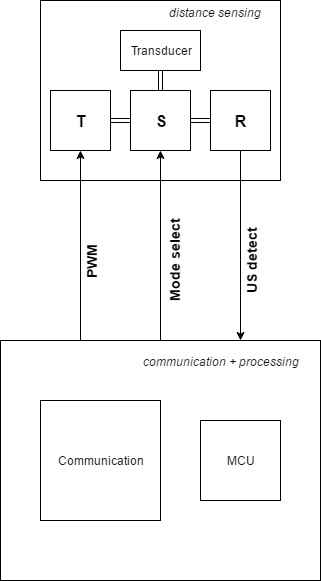
\includegraphics[width=0.5\textwidth]{Figures/integration.png}
\caption{Data link between the distance sensing system and the rest of the module}
\label{fig:int}
\end{figure}

Figure~\ref{fig:int} shows the data link between the distance sensing module described in this paper and the other systems in the module.
The figure shows:

\begin{itemize}
\item
\textbf{T} The transmitter circuit as described in section~\ref{chap:trans}.
\item
\textbf{R} The receiver circuit as described in section~\ref{chap:receiver}.
\item
\textbf{S} The switching circuit witch switches the transducer between the transmitter and receiver circuit.
\item
\textbf{PWM} \SI{40}{\kilo\hertz} \SI{50}{\percent} PWM wave generated by the microcontroller (MCU). This wave is amplified by the transmitter circuit to drive the ultrasonic transducer.
\item
\textbf{Mode select} Control signal from the MCU which selects the desired mode: transmit or receive. This is a \SI{5}{\volt} signal which switches the bilateral switches.
\item
\textbf{US detect} Data signal which tells the microcontroller if a ultrasonic pulse is received. This signal has two levels: \SI{5}{\volt} not receiving and \SI{0}{\volt} receiving.
\end{itemize}

These data connections, together with the power rail connections, connect the distance sensing module to the other systems in the module.
The MCU decides when an ultrasonic pulse has to be sent and actives the corresponding signals: the PWM signal to generate the signal needed to drive the transducer and the mode select signal to select the transmitter mode.
When the communication module receives an RF message from another Zebro telling it an ultrasonic pulse is incoming the MCU selects the receive mode and listens to the $US_{detect}$ signal.
How these data links are connected is explained in section~\ref{sec:proto_circuit}.

\section{Prototype circuit}
\label{sec:proto_circuit}

In appendix \ref{Appendixcircuits} is the total ranging circuit visible. This includes: the transmitter circuit, the switching circuit, the receiver circuit and the desired voltages together with some connectors. The modifications discussed before in section \ref{chap:mod} are all implemented in the circuits. When the circuits were ready, the layout of the printed circuit board was made to get a working naked prototype out of the PCB milling machine. The PWM signal as mentioned in the section before is the PWM40kHz signal in the circuit, the mode select signal is the ON/OFF signal in the circuit and the US detect signal is the output signal of the circuit.
Since all the components are known now, a bill of materials is made and visible in appendix \ref{AppendixBOM}
The total costs of all the components for a ranging circuit sums up to \euro11,57 per circuit.


\section{Module housing and antenna}
\label{sec:antennamech}

\begin{figure}[H]
\centering
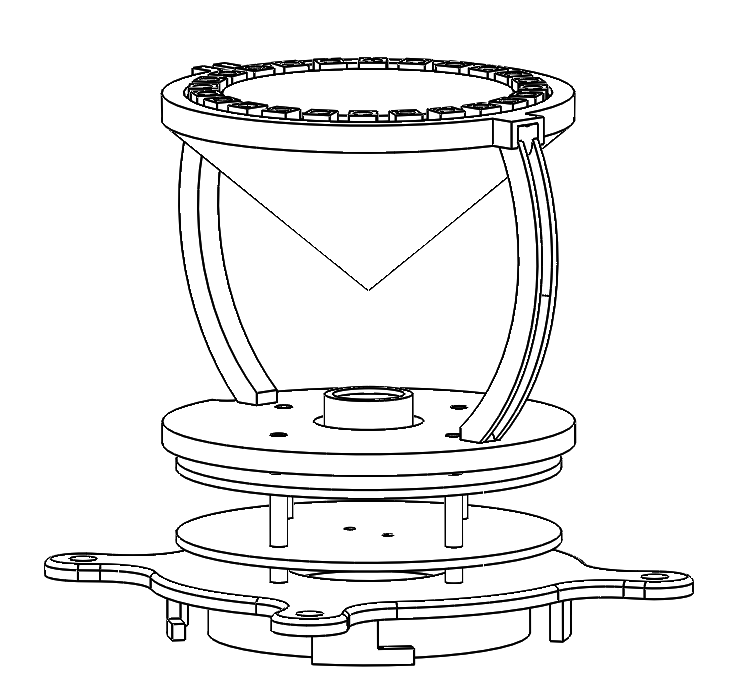
\includegraphics[width=0.8\textwidth]{Figures/prototype_ant.PNG}
\caption{3D model of the module prototype}
\label{fig:proto_module}
\end{figure}

To mechanically fasten the module to the Zebro a twist lock connection is required as described in the deci Zebro interface document~\cite{DeciSpecs}.
The system PCB stack is connected to the twist lock with four M3 risers.
The ultrasonic transducer is placed on the top PCB and slides in the antenna base plate.
The antenna base plate is placed on top of the PCB stack by connecting it to the M3 risers.
An 3D overview of the final module prototype is given in figure~\ref{fig:proto_module}.

The current prototype is kept modular.
The size, height and number of PCBs in the stack can change freely as long as they have the 4 M3 holes required to connect to the risers.
This makes sure last minute changes in the PCB design do not influence the design of the other prototype parts such as the twist lock connector.

\section{Naked prototype PCB}

 Visible in figure \ref{fig:naked_pcb}, is the print layout of the naked prototype PCB. It is taken into account that it is just a prototype. So to make the PCB as small as possible is not the biggest concern. The main concern is that it is a PCB that is easily to solder by hand, and if there are small failures in the board, it could be easy fixed. Also is taken into account that the components are placed in is logically. So the power circuits are at the top left side of the PCB, the transmitter circuit is at the left bottom side, with in the middle of the PCB the bilateral switch and on the right side the receiver circuit.

\begin{figure}[H]
\centering
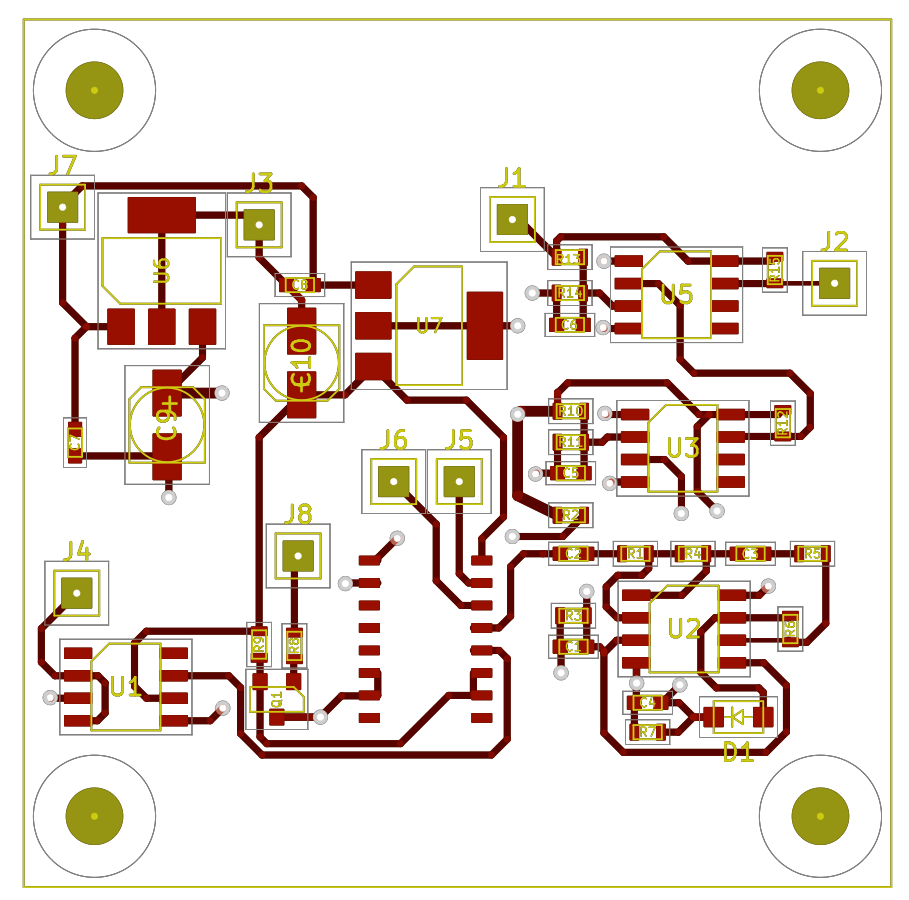
\includegraphics[width=0.6\textwidth]{Figures/Total_circuit.png}
\caption{Top layer of the naked proto PCB}
\label{fig:naked_pcb}
\end{figure}


\section{Problems during integration with communication system}
\label{sec:delay}
When testing the communication system the delay between giving the command to transmit a message an actually transmitting the message was found to be higher than expected.
During the concept design it was assumed that the RF message would be transmitted, and arrived at the other Zebro, instantaneous.
Test of the communication system showed that there is a delay of roughly \SI{6}{\milli\second} before the message was actually transmitted after the command was given.
This delay is likely due to the processing actions undertaken by the Digimesh modules to assure high mesh network communication performance.

The first problem this gives is a error of \SI{6}{\milli\second} in the measurement of $\Delta t$ (see figure~\ref{fig:ultra1}) since the ultrasonic pulse is now transmitted \SI{6}{\milli\second} before the RF message.
This gives an distance measurement result that is roughly \SI{2}{\meter} lower than the actual distance between the Zebros.

The second problem is that when the distance between the Zebros is low the ultrasonic pulse will now reach the other Zebro before the RF message does.
This means that the Zebro has not yet started the TDOA measurement since the RF message marks the start of the TDOA measurement.
The delay is \SI{6}{\milli\second} in which the ultrasonic pulse travels a distance of roughly \SI{2}{\meter}.
Thus when the distance between Zebros is smaller than \SI{2}{\meter} the ultrasonic pulse will arrive before the RF measurement thus resulting in a failed measurement.

Luckily the delay is roughly constant, it has a deviation of plus minus \SI{1}{\milli\second}, which makes it possible to work around this delay.
It is possible to:

\begin{itemize}
\item
Take the delay into account when calculating the distance form the measured $\Delta t$ by adding the delay to the measured $\Delta t$
This option provides no solution for the second problem: an ultrasonic pulse arriving before the RF message.
This means, when using this option, measurements cannot be done when the distance between Zebros is smaller than \SI{2}{\meter}.
\item
Adding the same delay to the transmission of the ultrasonic pulse such that the RF message and ultrasonic pulse are again transmitted simultaneously.
\item
Allowing both the RF message and the ultrasonic pulse to function as the $t_{0}$ timestamp for the TDOA depending on which arrives first.
This means that when the ultrasonic pulse arrives first we will measure the time difference between the arrival of the ultrasonic pulse $t_{0}$ and the arrival of the RF pulse.
Using the known value of the delay we can than calculate the distance between Zebros even if the ultrasonic pulse arrives before the RF message.
\end{itemize}

An attempt is made to implement the third option.
This option works for all distances, unlike the first option, and does not require the delay on the microcontroller the second option needs.
Implementing the delay on the microcontroller means that the microcontroller cannot undertake an other action during the \SI{6}{\milli\second} delay.
This would slow down the microcontroller and thus the system.

The implementation of this option is not discussed in this thesis since it is undertaken in the last 2 weeks of the bachelor end project after the deadline of the thesis.
We discuss the problem here since it will be included in the recommendations sections and it will influence the prototype testing phase as discussed in the next section.
